\section{Term-Template: Rewriting Metafunction Applications}

Since metafunction applications have the following shape - `(metafunction-name term-template ...)` these can be detected quite trivially given a list of defined metafunctions. 

\subsection{Rewriting Algorithm}
Let $Mf$ be the set of metafunction names. Let $t$ be some term-template, \Visit{$t$}. 
\begin{itemize}
\item $t=$\TermSequence. Check if $t_1$ is \TermLiteral with $kind=$Variable and $v \in Mf$ and return \\ \ApplyMetafunction[$v$][$t$][false] handling annotations as described below; otherwise return $t$. 

$t$ may contain \texttt{InArg} and \texttt{MatchRead} annotations and they are modified in the following way:
\begin{itemize}
\item
\texttt{InArg} annotations are left intact. Signatures of both \texttt{TermSequence} and \texttt{ApplyMetafunctions} must match.
\item
\texttt{MatchRead} annotations can be safely removed. None of such variable assignments are used to generate $t$.
\end{itemize}
\end{itemize}
\subsection{Example}
The example shown in Figure \ref{transformation-term-mfapply} displays the transformation described above given a set of meta-function names only containing single \texttt{set-contains?}. Since the first element of \texttt{TermSequence} is a \texttt{Variable} term-template with suitable name, an additional \texttt{MetafunctionApplication} term is added.

\begin{figure}[H]
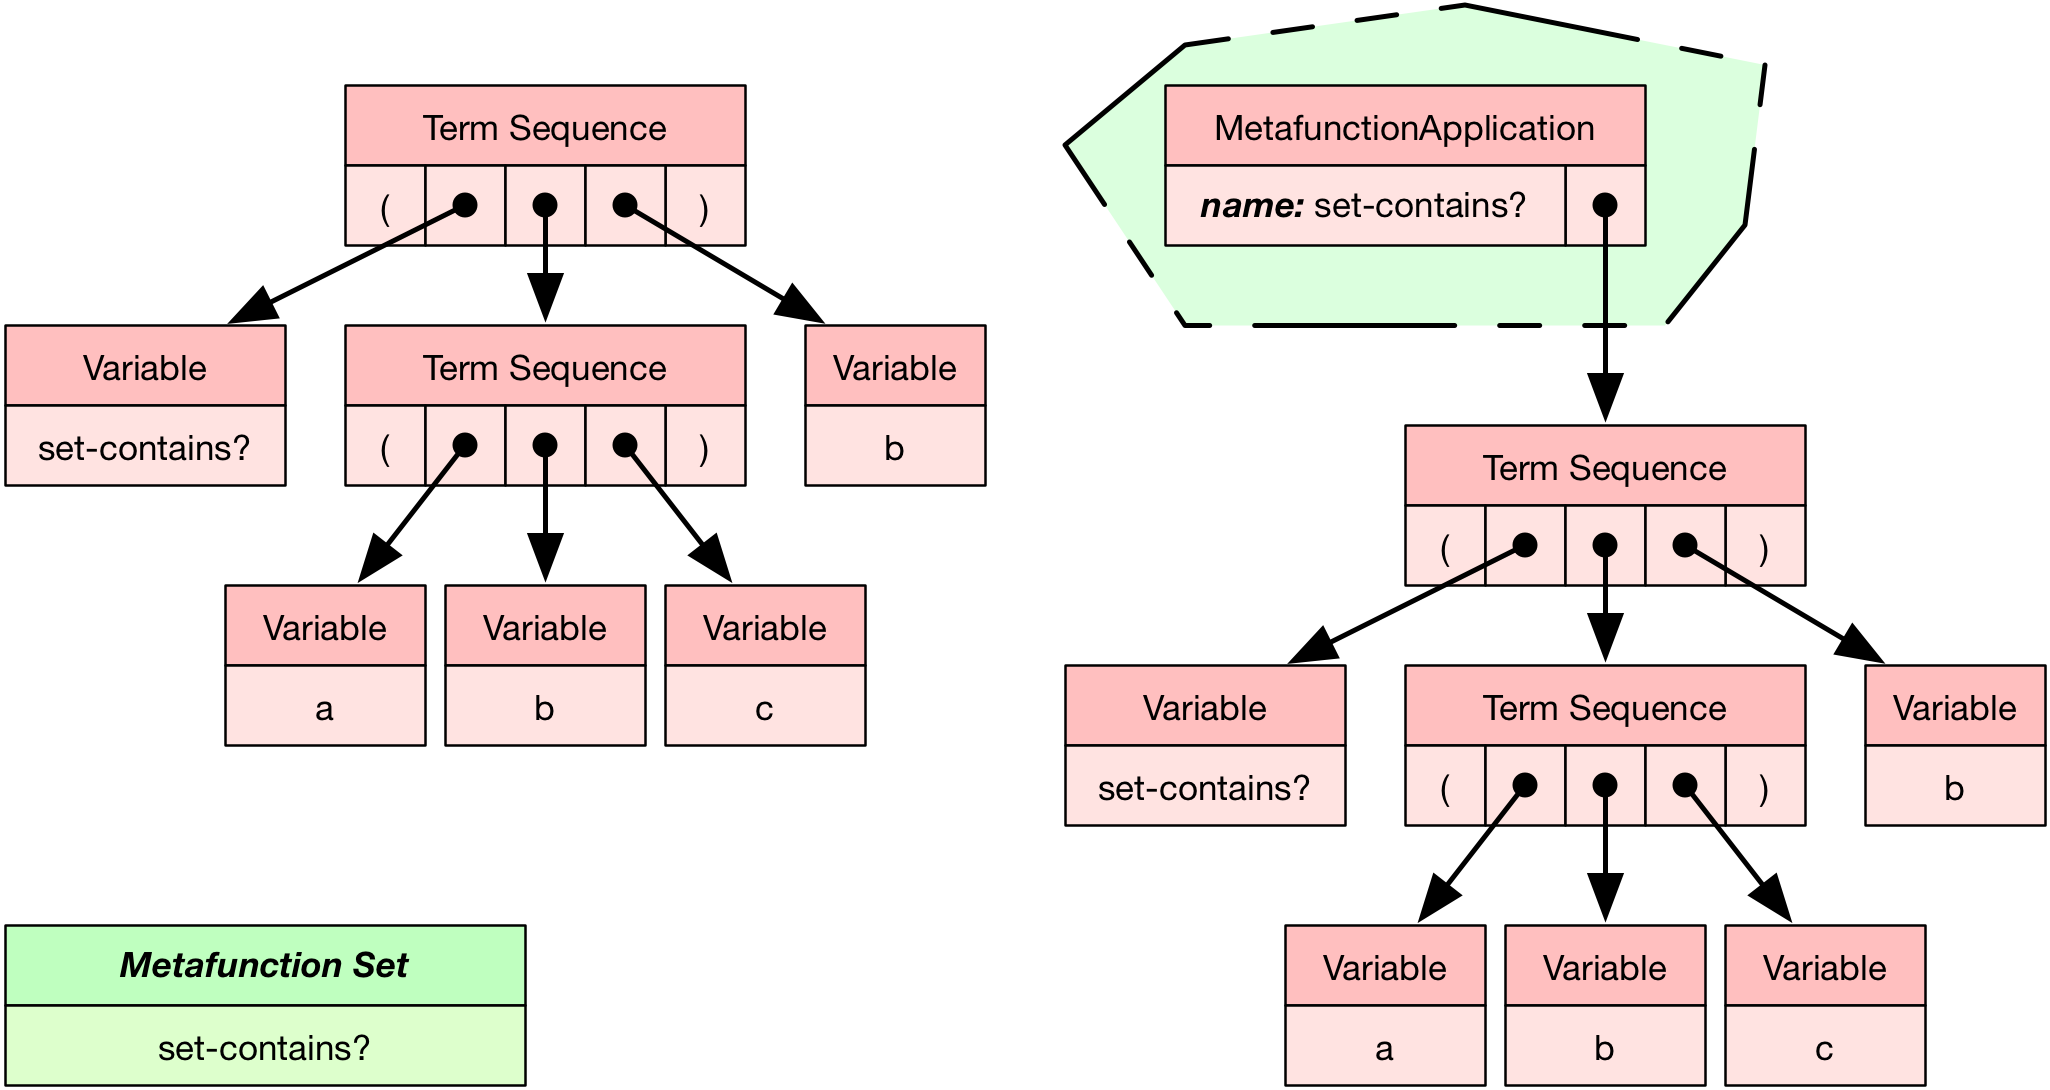
\includegraphics[scale=0.20]{transformation-term-mfapply.png}
\caption{Term-template before and after applying metafunctions.}
\label{transformation-term-mfapply}
\end{figure}
